\documentclass[10pt,letterpaper]{article}

\usepackage{booktabs}
\usepackage{caption}
\usepackage{subcaption}
\usepackage{setspace}
\usepackage{hyperref}
\usepackage{multirow}
\usepackage{minted}
% \usepackage{lineno}
% \linenumbers
\usepackage{pslatex}
\usepackage{apacite}
\usepackage{amsmath}
\usepackage{graphicx}
\usepackage[margin=1.0in]{geometry}

% \doublespace

\title{Analysis of the Simple Harmonic Oscillator \\ 
    {\small A foundational dynamical system}
}
\author{{\bf Matthew A.~Turner}}
\date{April 8, 2017}

\begin{document}

\maketitle

\section{1-dimensional simple harmonic oscillator: free and damped}
\label{sec:1d}

The simple harmonic oscillator is one of the first problems solved using
Newton's third law, $F=ma$. Usually this problem is framed as finding the
1-dimensional position of a mass on a spring, where the spring hangs from
a fixed surface with a mass on the other end.
The force is given by Hooke's law, which says that the restoring force 
of a spring is proportional to the distance from equilibrium, $x$, giving
$F = -k x$, where $k$ is the spring constant. Since $a$ is the second 
time derivative of position, Newton's third law can be written

\begin{align*}
    -k x &= m \ddot{x} \\
    \ddot{x} + \omega_0^2 x &= 0
    \label{eq:free-sho}
\end{align*}

\noindent
where $\omega_0 = \sqrt{k/m}$ is the \textit{angular frequency} of the motion,
or the number of cycles per second. $x$ is often referred to as ``displacement.''
In the case of a spring, $\omega$ is the 
rate at which the mass goes from its minimum displacement to its maximum 
displacement then returns to its minimum displacement. Because
sine and cosine have the negative of themselves as their second derivatives,
either can represent $x$ and as a solution to \ref{eq:free-sho}

\begin{subequations}
    \begin{align}
        x & = A \sin(\omega_0 t - \delta) \\
        x & = A \cos(\omega_0 t - \phi)
    \end{align}
\end{subequations}

\noindent
Note these are are identical if $\delta - \phi = \pi / 2$. 

The damped harmonic oscillator adds a damping force to Newton's third law,
$F_d = -b \dot{x}$. Damping effects, such as friction or air resistance,
are always proportional to velocity. Now the equation of motion is

\begin{align*}
    m \ddot{x} + b \dot{x} + k x & = 0 \\
    \ddot{x} + 2\beta \dot{x} + \omega_0^2 x & = 0
    \label{eq:damped-sho}
\end{align*}

\noindent
where $\beta = b/2m$.
Now to solve the equations of motion, we consider the solution $x = e^{rt}$.
Substituting we find 

\begin{align*}
    r^2 e^{rt} + 2 \beta r e^{rt} + \omega_0^2 e^{rt} & = 0 \\
    r^2 + 2 \beta r + \omega_0^2  & = 0
\end{align*}

\noindent
Thus,

\begin{align*}
    r = -\beta \pm \sqrt{\beta^2 - \omega_0^2}
\end{align*}

\noindent
There are three physically meaningful classifications of $r$: 
$r = -\beta$, $r$ is real-valued ($\beta^2 > \omega_0^2$), or 
$r$ is complex-valued ($\beta^2 < \omega_0^2$). These are referred to as
critical damping, overdamping, and underdamping, respectively. In the 
critical or overdamped cases, all periodic behavior is removed from the system
and the displacement goes directly to zero without switching sign. In the
underdamped case, there is quasi-periodic behavior as the displacement 
oscillates around zero, eventually settling to $x=0$. This is visualized 
in the phase diagrams below.

\subsection{Phase diagrams}
\label{sub:phase-diagrams}

In the simple harmonic oscillator, the relevant state variables are the 
displacement, $x$, and the velocity $\dot{x}$. First we will consider the
free harmonic oscillator, where the damping $b=0$. Taking the solution 
$x(t) = A \sin(\omega_0 t - \delta)$, we find 
$\dot{x}(t) = A\omega_0 \cos(\omega_0 t - \delta)$. We can square both equations
and divide the right-hand constants to get

\begin{align*}
    \frac{x^2}{A^2} & = \sin^2(\omega_0t - \delta) \\
    \frac{\dot{x}^2}{A^2\omega_0^2} & = \cos^2(\omega_0 t - \delta)
\end{align*}

\noindent
Adding the two equations and using the 
relation $\sin^2(\theta) + \cos^2(\theta) = 1$ we recover the equation for
an ellipse

\begin{align*}
    \frac{x^2}{A^2} + \frac{\dot{x}^2}{A^2 \omega_0^2} = 1
\end{align*}

\noindent
A few phase diagrams for the free harmonic oscillator are shown in Figure \ref{fig:free}

\begin{figure}[h!]
\begin{center}
    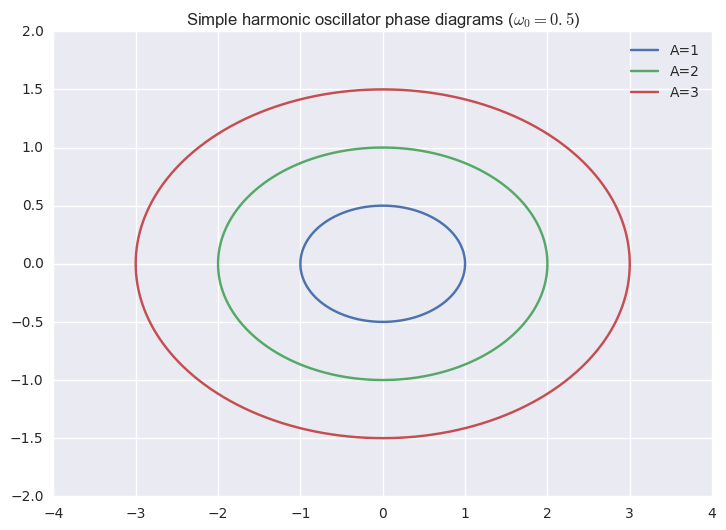
\includegraphics[width=0.6\textwidth]{figures/free-sho.png}
\end{center}
\caption{Phase portrait for some values of $\beta$ for the underdamped harmonic oscillator}
\label{fig:free}
\end{figure}

\begin{figure}[h!]
\begin{center}
    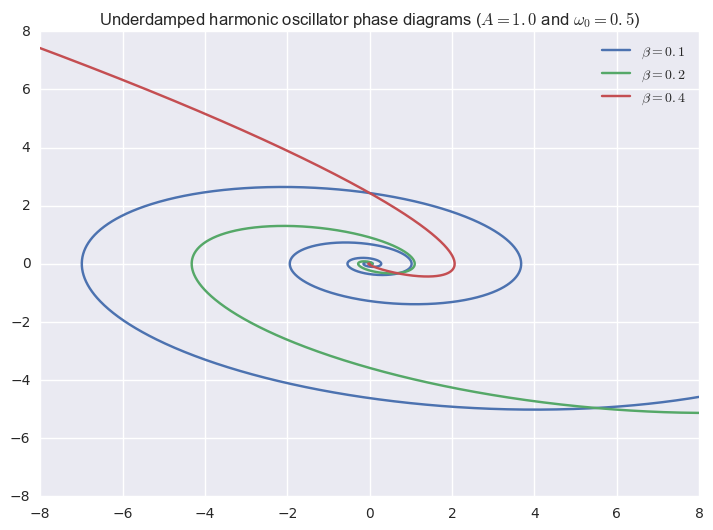
\includegraphics[width=0.6\textwidth]{figures/underdamped-sho.png}
\end{center}
\caption{Phase portrait for some values of $\beta$ for the underdamped harmonic oscillator}
\label{fig:underdamped}
\end{figure}

In the case of the underdamped harmonic oscillator, it can be shown that
the solution is $x(t) = Ae^{-\beta t}\cos(\omega_1 t - \delta)$, where
$\omega_1 = \sqrt{\omega_0^2 - \beta^2}$. Using the chain rule for derivatives,
we find $\dot{x}(t) 
= -Ae^{-\beta t} (\beta \cos(\omega_1 t - \delta) 
+ \omega_1 \sin(\omega_1 t - \delta))$. A few phase diagrams for the underdamped
harmonic oscillator are shown in Figure~\ref{fig:underdamped}.



\rule{\textwidth}{1pt}

Thornton, S. T., \& Marion, J. B. (2004). \textit{Classical Dynamics of Particles and Systems}.
(5th ed.). Belmont, CA. Thompson Brooks/Cole.
\end{document}
